\documentclass[12pt, letterpaper]{article}

%% My used library
\usepackage{float}
\usepackage{subcaption}
\usepackage{graphicx}
\usepackage{booktabs}
\graphicspath{{Figs}{Figs/}}


\title{My first LaTeX document}
\author{Hubert Farnsworth\thanks{Funded by the Overleaf team.}}
\date{August 2022}
\begin{document}
\maketitle
We have now added a title, author and date to our first \LaTeX{} document!\cite{chen2018}


\section{Introduction}\label{sec1}
Suicide is a significant cause of death worldwide. Only In USA approximately 46,000 people committed suicide in 2020. Many countries the second highest cause of death among teenagers and younger adults is suicide. Suicide and depression are major health hazards, resulting in the death of one person every 40s globally1,2. More than 300 million people worldwide experience depression and annually, ~800,000 people die by suicide.. They are complex and intertwined phenomena: ~4\% of individuals diagnosed with depression commit suicide, and more than half of the persons who attempt suicide meet the criteria of depression. Hence, depressed individual posses suicidal tendency. To what extent of depression level triggers suicidal risk. Conventional interview-based diagnosis is insufficient to accurately predict a psychiatric status. Because more-often patients prefer not to disclose their emotions, often reluctant to seek help from psychotherapists, or clinic doctor. Also, It is hard to quantify the level of depression during suicidal attempt. It may varies based on various factors like society, religion, family bonding, emotional maturity and many others factors. Due to lack of confidence, fear of death, religious obligations, and societal stigma against this act, even severe depressed person may not consider making an attempt at suicide.

 

It is common phenomenon that emotionally distressed individual is hiding their depression. But at the same time seeking empathy consciously or unconsciously in the social sites like twitter, reddit and facebook \cite{chen2018, park2013perception, de2013predicting, xu2016contribution, burnap2015machine}. We can determine severity level of depression by analyzing social media activities. Clinically depression and suicide prediction methods rely on self-reported measures such as predefined categorical questionnaires and interviews, which can be too subjective; and people with depression and suicidal ideation may not be honest about expressing their thoughts. we present machine learning and statistical prediction models for depression and suicide risk prediction. our research focus on detection of suicidal tendency within a depressed person’s post. Find out important features, explore different facts and hidden underlying information for depression and suicide.  

\section{Literature Review}
In india, USA and many other countries significant number of people die because of suicide. \cite{havigerova2019text, singh2022startling}. Depressive disorder patients show some degree of suicidal behaviour and may lead to severe consequences. \cite{vuorilehto2006suicidal, mcgirr2007examination, hawton2013risk} Several studies showed that depression depression patients are very prone to suicidal attempt.  
Extensive research has been conducted before about depression and suicide. In 2020 Chancellor et. al conducted systematic literature review of the mental health status prediction using social media data \cite{chancellor2020methods}. More than 75 studies were taken into consideration between 2013 to 2018. It provides a detailed overview of data collection sources, data annotation methods, pre-processing and feature selection, model selection followed by accuracy estimation, cross validation and models’ benchmarks for mental illness. In 2022 Zhang et. al claimed that 399 scientific research papers were reviewed and mental illness related research is increasing gradually \cite{zhang2022natural}. There were other review papers on these two issues in which similar topics are analyzed by Castilla in 2020 \cite{castillo2020suicide}  and Malhotra 2022 \cite{malhotra2022deep}. All of these review based research studies analyzed mostly Text data, and discussed NLP tools and techniques. In some research multimodal data samples are used such as: Text samples from the social website and shared images from Instagram. Along with status of the social website and Electronic Health Record (EHR) has also been taken into consideration \cite{zheng2020development, mann2020see}. Audio and audio visual impact on individuals to detect depression also has been studied in some papers \cite{ye2021multi, he2022deep}. In 2021 Lang He et. al conducted research of Audio visual features \cite{he2022deep} aiming how facial expression and voice can be used as an input features to determine mental illness effectively. Apart from reviewing previous research articles, Martinengo reviewed 69 apps in 2019 that provides suicide preventive solutions and support \cite{martinengo2019suicide}. Most of these apps have emergency calling features that can support mental patients over phone or app. In this study we will be focusing on the text based features only for mental illness and suicidal pattern detection. Text based expression depicts mental illness more clearly compared to other symptoms and is dominant among researchers to detect mental issues effectively.


Dataset
Text based Suicide and depression detection classification task uses NLP techniques and methodologies which are highly dependant on the quality of dataset, accurate annotation and size of samples. These samples are mostly collected from Twitter, Reddit \cite{tadesse2019detection}, facebook, weibo etc websites donated by these institutions or other researchers. Several researchers contributed dataset and made it available publicly \cite{rissola2020dataset}. In 2021 the Computational Linguistics and Clinical Psychology CLPsych 2021 workshop organized a Task challenge for detecting suicidal risk \cite{macavaney2021community}. It facilitated participants providing sensitive authentic dataset on the problem of predicting suicide risk from social media Twitter. The dataset for the task includes information who attempted suicide or succeeded along with some control who have not. [The University of Maryland Reddit Suicidality Dataset, Version 2]\cite{shing2018expert} Various researchers consulted with the practitioner professional psychiatrist to annnotate the dataset and segregated into several categories to determine degree of intensities of suicidal risk \cite{gaur2019knowledge}. \cite{lopez2022exploring} This research study used Twitter post collection API for collecting Tweets and collected Tweets of size 2509 were obtained, of which 216 post were found relevant by 3 Expert psychologists evaluators. Furthermore, using LIWC, dictionary of the Linguistic Inquiry and Word Count \cite{pennebaker2001linguistic}, which is a linguistic feature analysis software that calculates the degree of positive and negative emotions across a wide spectrum of texts, Tweets were evaluated and results are statistically presented. 

Many researchers also employ interrogative questionnaire-based datasets that were created after speaking with the patients in an interview session. 

Structured Instrument for measuring Severity rating Scale 
From the very beginning questionnaire based intensity measurements for depression and suicidal tendency was developed. Depression and suicidal intensity measurements scale are applied for setting the questionnaire during the interrogation. This process provides weights to answers replied by individuals. Most renowned scales are PHQ-9, BSS \cite{beck2000weisman}, DSM-5, DASS-21 \cite{havigerova2019text}, Columbia Suicide Severity Rating Scale (C-SSRS) \cite{posner2011columbia, joiner1997modified} etc.  Most of these scales are based on predefined questions and answers. \cite{havigerova2019text, beck1961inventory, kroenke2001phq, tolentino2018dsm, kliem2017german, eke2010hamilton}. These scales are mostly specified questions and multiple choice questions and answers have weight 1~5 and according to the feedback from the user severity of symptoms are decided. Then statistical Machine Learning models are applied to investigate patterns \cite{shen2020detecting}. \cite{shen2017depression} The Beck's Depression Inventory \cite{beck2000weisman} consists of 21 questions regarding the users' physiological and mental states. Another example is the CES-D Scale \cite{radloff1977ces}, which has 20 questions concerning users' sleep patterns and guilty feelings. Users must either rate the severity of their circumstances in response to the questions, which either offer many answers with varying scores, or both. According to the scale of the overall score, the degree of depression is identified. In contrast, the Diagnostic and Statistical Manual of Mental Disorders (DSM) \cite{whooley2014diagnostic} offers nine different types of depressive indications, including low mood and impaired interest. Before making a final judgment, clinicians typically determine if these symptoms have been prevalent throughout time.

In \cite{vuorilehto2006suicidal} research study conducted in the City of Vantaa, Finland, for the age group of 20 to 69 years with 1119 primary-care patients using (PRIME-MD) questionnaire. Suicidal behaviour was investigated and present suicidal ideation was measured with the Scale for Suicidal Ideation (SSI) and afterwards suicide attempts were evaluated based on medical records. Survey is conducted on specific demographics of population, Mostly statistical machine learning methodologies are applied to determine risk, features and intensities within collected samples [Detecting risk of suicide attempts among Chinese medical college students using a machine learning algorithm]. In [Detecting risk of suicide attempts among Chinese medical college students using a machine learning algorithm] 4,882 medical students were surveyed on the basis of demographic and clinical records via WeChat app. In [Knowledge-aware Assessment of Severity of Suicide Risk for Early Intervention] collected dataset of 2181 redditors post which contains posts related to suicidal ideation, behavior, or attempt. Then assisted by professional practitioners, the psychiatrists prepared a dataset of only 500 redditors using tool called C-SSRS \cite{posner2011columbia}. \cite{vuorilehto2014method} Within the Vantaa Primary Care Depression Study (PC-VDS, 91 patients) and the Vantaa Depression Study (VDS, 153 psychiatric out-and 41 inpatients), suicidal ideation was assessed with the Scale for Suicidal Ideation (SSI), Hamilton Depression Scale (HAM-D) item 3 and Beck Depression Inventory (BDI) item 9, and by asking whether patients had seriously considered suicide during the episode. The positive and negative predictive values (PPV, NPV) for suicide attempts during a six-month follow-up were investigated. 


These standards have been successfully validated and used for many years in real-world situations, without a doubt. Till date many researchers are using these scales to determine suicidal symptoms and abuse \cite{li2022association}. However, because it took the DSM 12 years to grow from DSM-IV to DSM-V, it may take some time for these criteria to be strictly updated. As a result, they might not completely encompass new behaviors and symptoms like those that are communicated by the current social media.


\cite{shen2017depression} We, particularly the depressed users, almost cannot exist in this new world without social media. Thus, studies on the internet habits of individuals who are depressed began. Park et al. [2012] used real-time mood data from Twitter users as part of their early research to examine how language is used to describe melancholy moods. In order to investigate the depressed behaviors of 14 active Twitter users, Park et al. [2013] conducted face-to-face interviews with them. The most recent study, by Xu et al. [2016], sought to explain how online users debate topics connected to depression from the standpoint of social networks and language patterns. With the aforementioned research, social media depression detection was made possible. The possibility of detecting and diagnosing serious depressive illnesses via social media was investigated by Choudhury et al. in 2013.

Modality of Dataset
Social media dataset are mostly Text data which needs data preprocessing, cleaning, feature extraction and data mining related NLP tasks. Machine learning and Deep Learning models are particularly used for Text classification and ML for feature selection or extraction in several studies \cite{castillo2020suicide, chancellor2020methods, zhang2022natural}. These extensive reviews reveal Deep learning methods receive more attention and perform better than traditional machine learning methods whereas in some cases when extracted or filtered features are fit into training process models are able to perform better. NLP techniques are applied for the annotated dataset collected from Twitter, Reddit, Facebook, instagram, Weibo \cite{wang2020depression} etc. After that various deep learning and machine learning models are trained for classification of suicide and depression. Then trained models are applied to determine the correct class of given text. \cite{malhotra2022deep} Provided a through investigation about passed research techniques, features, datasets, and performance metrics. \cite{zhang2022natural, chancellor2020methods} Among Several Deep Learning approaches most successful NLP classifier for segregating Depression and suicidal task are CNN, LSTM, GRU, XLNET, BERT, Variants of BERT RoBERTa and variants of CNN such as: CNN-BiLSTM etc \cite{aldhyani2022detecting, wang2020depression, shetty2020predicting} . 


In 2017 Shen et. al [Depression Detection via Harvesting Social Media: A Multimodal Dictionary Learning Solution] Collected several forms of features comprised of six chorots, namely, social network features, user profile features, visual features, emotional features, topic-level features, and domain-specific features and prepared a feature rich dictionary. This multimodal depressive dictionary learning model was used to detect the depressed users on Twitter using machine learning models. 

  

In \cite{aldhyani2022detecting} proposed suicidal ideation detection system using publicly available Reddit datasets in Kaggle Website comprised of 232,074 post annotated for binary classification as suicidal or non-suicidal. 

Apart from the Deep learning model n-gram Traditional feature retrieve based analysis conducted in some research papers. Most dominant approaches are TF-IDF, Word2Vec, XGBoost, SVM, Random Forest, other regression ML models are classifiers and LIWC \cite{pennebaker2001linguistic}, LDA, Bigram etc are used as features analysis tools \cite{tadesse2019detection}. Typical word embedding approaches TF-IDF and Word2Vec, and CNN–BiLSTM are applied in  \cite{aldhyani2022detecting}. Using LIWC features, XGBoost ML together surpasses the accuracy of CNN–BiLSTM in  \cite{aldhyani2022detecting}. Others have used machine text Summarization based feature extraction strategy followed by classification for depression detection is applied in \cite{zogan2021depressionnet}. 


\cite{burnap2015machine}built a set of baseline classifiers using lexical, structural, emotive and psychological features extracted from Twitter posts. Then baseline classifiers are updated by building an ensemble classifier using the Rotation Forest algorithm and a Maximum Probability voting classification decision method. 
[Methods in predictive techniques for mental health status on social media: a critical review]
This paper provided an excellent overview of 75 studies in between 2013 and 2018 outlining the methods of data annotation for mental health status, data collection and quality management, pre-processing and feature selection, and model selection and verification. 

Other Tools or Methods
Apart from the NLP based dataset classification and Questionnaire based Machine Learning or statistical model approaches there are some sites, helpline numbers and apps \cite{martinengo2019suicide} that contains various facts, statistics, tips, tools, healthline numbers and various ways to handle suicidal depression. [Suicidal Depression: Understanding It and Finding Help]
  


\section{Backgound}\label{sec2}


Suicidal risk estimation task and classification samples to determine suicidal risk within social websites and blogs, techniques are discussed before. According to suicidal category previous work has been done before. However, to what extent depression level triggers suicidal risk is not yet discussed before. Also it is difficult to determine since depression and suicide categorical variables are independent factor. There is not any underlying correlation. Several research conducted to segregate which post is suicidal and which one is depression various classifiers are proposed. Extensive work has been done to improve the classification accuracy by adopting most powerful vectorization techniques that uses cutting edge NLP models BERT and its various variants. Research has also been conducted on how much severity label of suicide within a post is studied. 
To detect various level of suicidal risk within the depressed person suicidal risk determinant AI classifier is created. After being detected with risk 

\begin{figure}[H]
  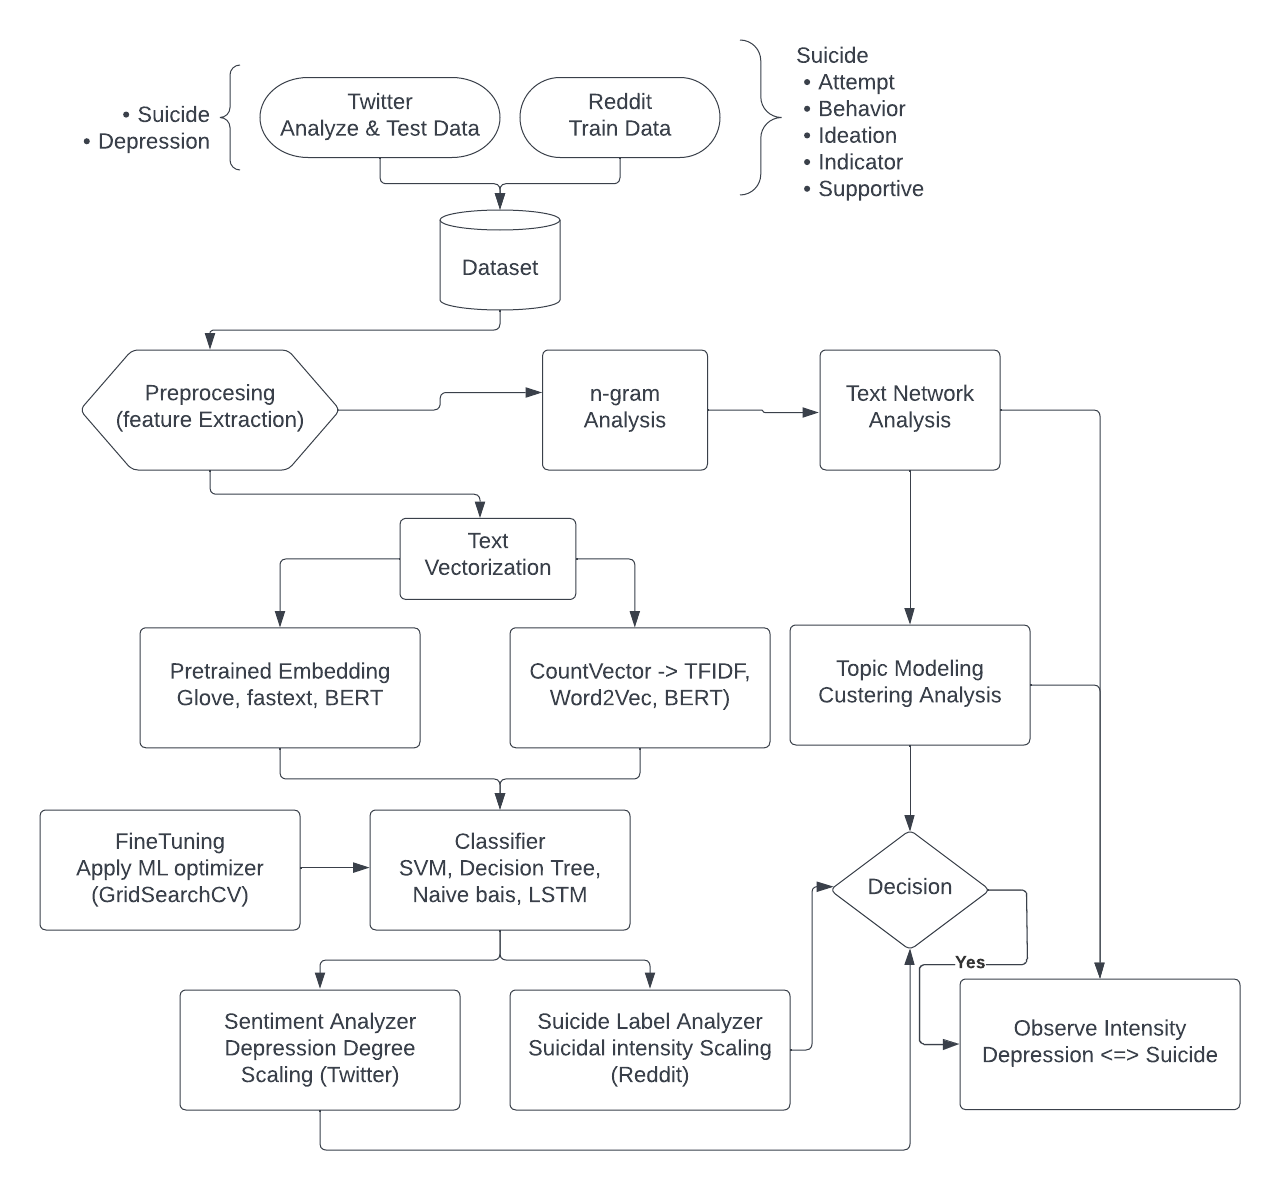
\includegraphics[width=0.8\textwidth]{res_diagram.png}
  \caption{A boat.}
  \label{fig:boat1}
\end{figure}

\section{Methodology}\label{sec2}

predictive model can provide AI support Depression and suicidal risk, this two occurrences’ implicit relationship is explored in this research.

 This classifier can classify and detect suicidal attempt within the conversation. Along with various machine learning algorithms, deep learning models are also applied to estimate the label accurately. Facebook also proposed a technique by which it can detect suicidal post in their site and can take necessary attempts. Though underlying techniques are not disclosed publicly. To estimate severity of suicidal tendency research is available but how depression affect suicidal attempt is not present yet. This holistic investigation is to aware and explore the factors and terms related between this two emotional states symptoms using NLP’s statistical techniques. 
Methodology
In this research we are only considering the text expression available in internet and open access dataset. In several research papers reddit dataset has already become a good estimator to determine depression and suicide. 

which is used to determine the depression intensity within a suicidal post. 
For training the classifier CSSR dataset is used which provides the suicidal risk classification dataset and has specific features belongs to specific category of suicidal risk. Trained classifier, detects the suicidal risk within reddit post which contains depression vs suicide category. Text is converted to meaningful feature vector then classifier is trained to determine depression degree within a suicidal post. From the observed result statistical analysis explained the degree of depression within a suicidal post can be estimated.  In our analysis we used different classifiers to determine the intensity and degree of depression within suicide tendency. 




\section{Results}\label{sec2}


First we cleaned the dataset by removing unwanted characters, symbols and stop words. Then further pre-processing is conducted which are followed for standard data cleaning process for NLP task. 


\begin{figure}[h!]
\centering
\begin{subfigure}{0.45\textwidth}
    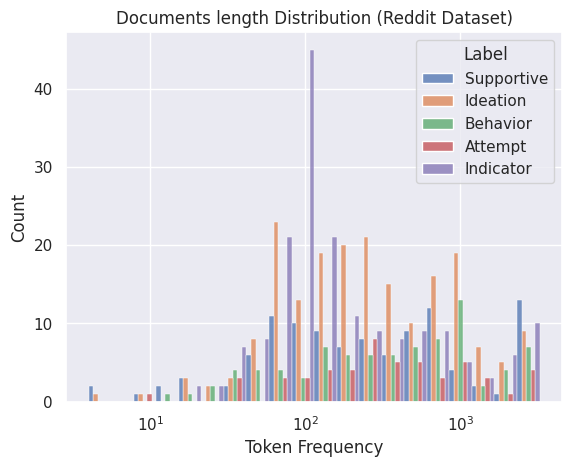
\includegraphics[width=\textwidth]{reddit_dist.png}
    \caption{First subfigure.}
    \label{fig:first}
\end{subfigure}
\hfill
\begin{subfigure}{0.45\textwidth}
    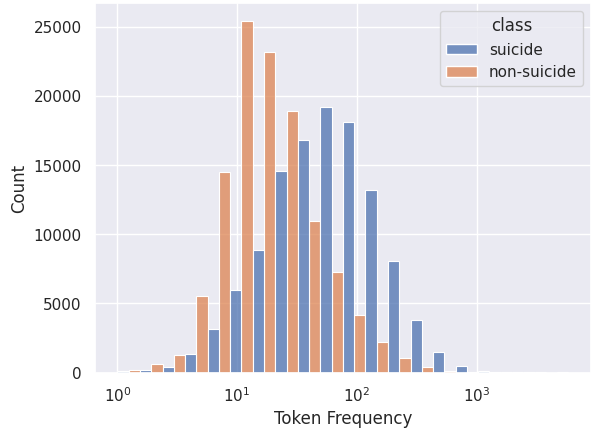
\includegraphics[width=\textwidth]{twitterdist.png}
    \caption{Second subfigure.}
    \label{fig:second}
\end{subfigure}
        
\caption{Subreferences in \LaTeX.}
\label{fig:figures}
\end{figure}


First we started our experiment with the length of document. We found a pattern that depression comments are tend to be smaller than depression class. Our main dataset distribution among depression and suicide class ratio is equal. But  depression class is usually shorter in length. Short sentence does not carry much terms and hence does not carry enough information to be classified confidently by classifier algorithms. Since, Class distribution among depression and suicide category ratio is equal in the dataset. We started reducing the numbers of samples based on document length. By reducing the samples based on numbers of tokens present in a document (see Figure). Documents length versus category frequency information is showed in this chart. This charts explains if we filter out the shorter comments suicide post become dominant class and depression post become outnumbered. The difference showed an exponential pattern as length of document increases. Filtering the class we have seen an interesting fact that depressed people does not want to comment very long. 

Then ngm analysis is conducted. 


They tend to use slang and abusive terms compared to suicidal attempt thinking people. Rather suicidal depressed people want to share their thoughts with others using longer post. 

\begin{figure}[H]
\centering
\begin{subfigure}{0.45\textwidth}
    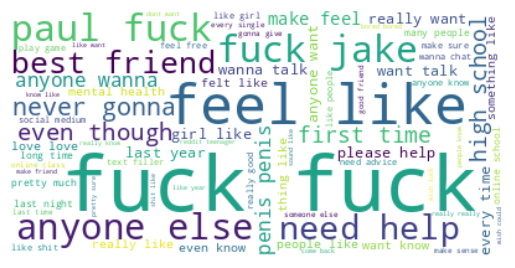
\includegraphics[width=\textwidth]{dep_wordcloud.png}
    \caption{First subfigure.}
    \label{fig:first}
\end{subfigure}
\hfill
\begin{subfigure}{0.45\textwidth}
    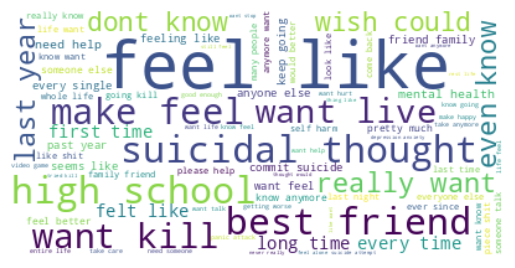
\includegraphics[width=\textwidth]{sui_wordcloud.png}
    \caption{Second subfigure.}
    \label{fig:second}
\end{subfigure}
\hfill
\begin{subfigure}{0.8\textwidth}
    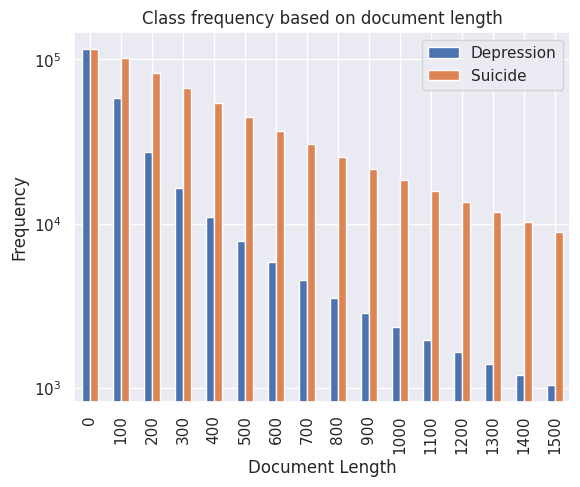
\includegraphics[height=7.5cm, width=\textwidth]{doc_len.png}
    \caption{Second subfigure.}
    \label{fig:second}
\end{subfigure}
        
\caption{Subreferences in \LaTeX.}
\label{fig:figures}
\end{figure}

Frequency based comparison between two categories is conducted. Main objective was to get top ranked words from Depression and Suicide corpus. After experiments we have seen There are similarities between the top ranked words those are occurring frequently. However, it does not reveals any clues of hypothetical relationships between the two category. To understand the term occurring frequently in two different classes scatterplot library is used for visual analysis.  



From the above two scenario we can see that there is a pattern that people used to say more slang and abusive words when they are depressed. It is also interesting that there are many words have high frequency such as depression or depressed but belongs to suicide class. 


One important fact is revealed here is that we can see although suicide, suicidal these words has high frequency in Suicide class but depression, depressed also occurred in parallel with high frequency. Here several experiments can be conducted for exploratory analysis with scattertext library for terms significance. However, this library is computationally heavy for larger dataset for visualization. Another drawbacks is this library have significant focus on the terms based analysis. We have used simple vectorization methods by which we can have greater control on dataset and experiments code. First bigram is analyzed with countvectorizer for both categories. The bigram frequency showed there are some common terms like “mental health”, “feel like”, “make feel”, “high school” etc. Hence, we started to understand its pattern in the corpus. For analysis we have considered ['high school', 'mental health', 'best friend', 'feel like', 'really want', 'suicide thought', 'friend family'] these bi-grams and wanted to explore its surrounding context for each category. We called this special bigrams since it showed importance in the suicidal and depression both categories. We want to analyze how these words have impact with its neighboring words. Tri-grams or above did not reveals much meaning information, mostly does convey some meaningful information and therefore excluded for further experimental consideration. 
\begin{table}[h]
\begin{center}
\begin{minipage}{174pt}
\caption{Caption text}\label{tab1}%
\begin{tabular}{@{}lllll@{}}
\toprule
Classifier & Precision & Recall & Accuracy & F1 \\
\midrule
Nearest Neighbors & 0.926 & 0.924 & 92.3896 & 0.924\\
RBF SVM & 0.942 & 0.924 & 92.3896 & 0.927\\
Decision Tree & 0.901 & 0.848 & 84.7793 & 0.856\\
Random Forest & 0.513 & 0.282 & 28.1583 & 0.167\\
Neural Net & 0.942 & 0.927 & 92.6941 & 0.929\\
AdaBoost & 0.905 & 0.898 & 89.8021 & 0.899\\
Gaussian Process & 0.940 & 0.921 & 92.0852 & 0.924\\
Naive Bayes & 0.923 & 0.918 & 91.7808 & 0.919\\
QDA & 0.931 & 0.909 & 90.8676 & 0.912\\
%\botrule
\end{tabular}
\footnotetext{Source: This is an example of table footnote. This is an example of table footnote.}
\end{minipage}
\end{center}
\end{table}
To explore the impact of special bi-grams on the samples, special bi-gram terms containing samples are filtered from dataset. Filter and segregate special bigrams dataset for each category then use the popular document ranking approach: countvectorizer → TFIDF vectorization → get (special bigram) features rank. Here ranking is the summation of total TFIDF score for any given feature. 
After that using lebel encoder bigrams are encoded as integers and then chord diagram is generated to find meaningful relationship within the samples between the bigram features.  


\begin{figure}[H]
\centering
\begin{subfigure}{0.8\textwidth}
    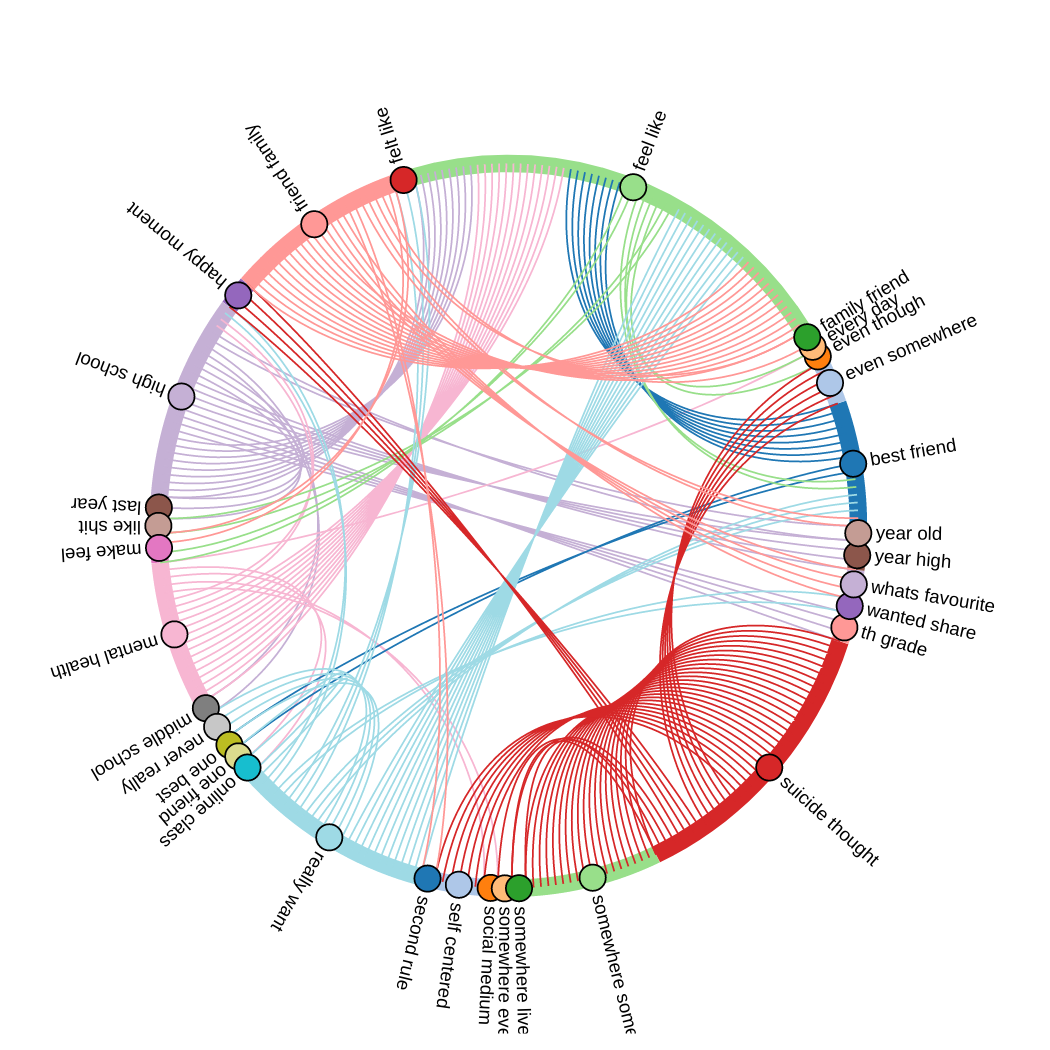
\includegraphics[width=\textwidth]{dep_chord.png}
    \caption{First subfigure.}
    \label{fig:first}
\end{subfigure}
\hfill
\begin{subfigure}{0.8\textwidth}
    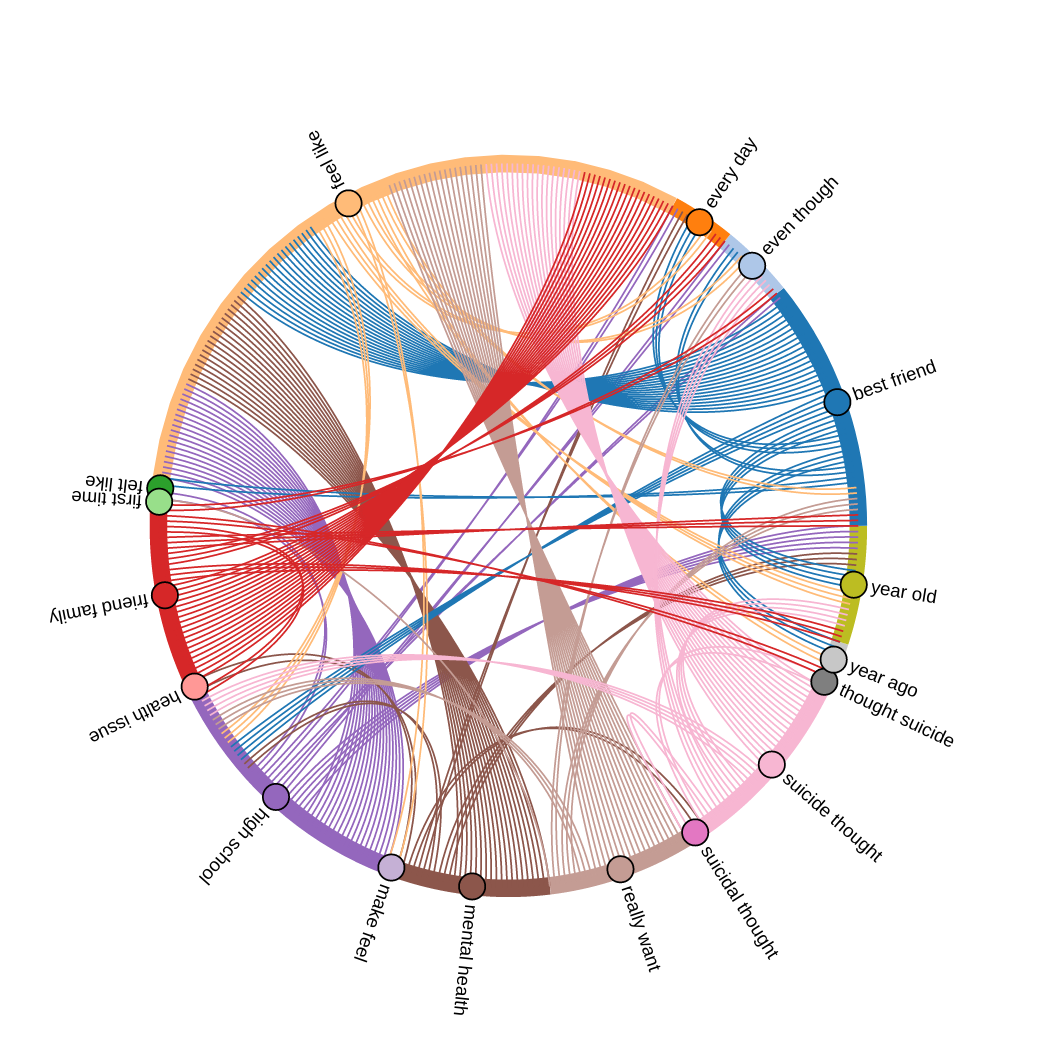
\includegraphics[width=\textwidth]{suicide_chord.png}
    \caption{Second subfigure.}
    \label{fig:second}
\end{subfigure}
        
\caption{Subreferences in \LaTeX.}
\label{fig:figures}
\end{figure}


From this two chord diagram interesting sentence can be inferred. Such as: from the depression class → self centered person is depressed → having suicidal thought → want to go somewhere to live → spend happy moments and so on. For the suicidal class category suicidal attempt thinking people → have mental health issue → they want to share though with high school friends → best friends → friends and family members → having suicidal thoughts and so on.  

However, it is difficult find such pattern in which we can determine the depression and suicidal thought. So far we found some pattern 1) short statements likely to be more depression category
2) Depressive statements tend to have slang
3) Suicidal thinking people’s post having very high frequency of “kill” “die” these type of words or phrases.

Someone may be in extreme depression but due to lack of confidence, fear, religion bindings, family trauma or social prohibited action, thinking about all, individual can not think about taking suicidal attempt. How much depression can trigger suicidal thoughts is an interesting question. 

For determining the suicide risk in various category there is dataset available publicly and improved by C-SSRS. However, how depression intensity triggers or affect suicide ideation or attempt taking is very crucial. 

To segregate the Reddit suicide dataset into different categories first we have created a classifier using different classification techniques. Since our objective is not making highly accurate classifier. We have used simple gridsearch technique of sklearn library and from a list of various classifiers applied on the dataset, we have chosen highest accurate classifiers to determine different label of suicidal risk. so that it can recognize the category. 

We have used classifiers "K Nearest Neighbors", "Linear and RBF SVM", "Gaussian Process", "Decision Tree", "Random Forest", "Vanilla Neural Net", "AdaBoost", "Naive Bayes" and so on. 

Using various set of parameters. From the result and experiments we found almost 60\% accuracy for SVM model. From various set of values of SVM we found degree=2, gamma=0.7, kernel=rbf
showed the highest accuracy. 

Using this classifier we have achieved almost 73\% accuracy for the Reddit “depression/Suicide” dataset. Since we want to segregate the suicidal attempt in depth hence segregation of suicidal dataset is important. It will provide a clear idea how the columbian suicidal category have impact over suicide class. 

1. We have used Reddit 500 post CSSR dataset
2. Pre-processed and get useful features
3. Use count vectorizer and TFIDF transformer to generate vectors for the dataset
4. Train a classifier to determine the categories 

To determine this we will use a dataset in which different level of depression and suicidal thoughts category is leveled. 

\begin{figure}[H]
\centering
\begin{subfigure}{0.45\textwidth}
    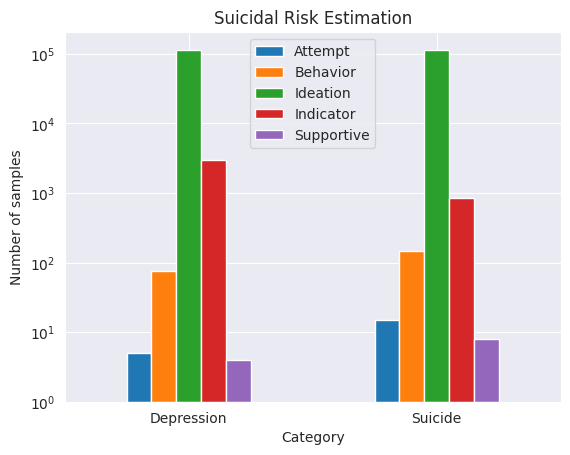
\includegraphics[width=\textwidth]{grid_svm.png}
    \caption{First subfigure.}
    \label{fig:first}
\end{subfigure}
\hfill
\begin{subfigure}{0.45\textwidth}
    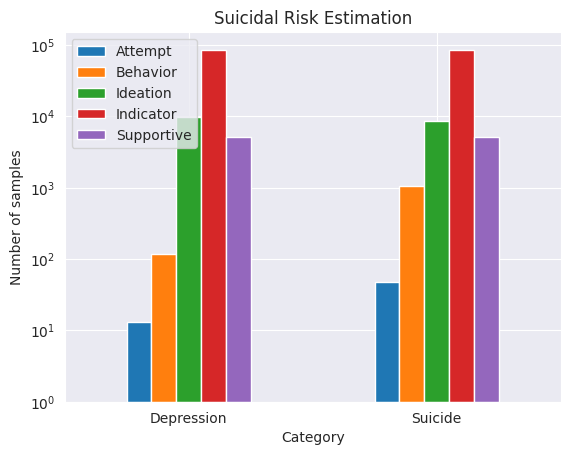
\includegraphics[width=\textwidth]{glove_vec.png}
    \caption{Second subfigure.}
    \label{fig:second}
\end{subfigure}
        
\caption{Subreferences in \LaTeX.}
\label{fig:figures}
\end{figure}


\begin{figure}[H]
\centering
\begin{subfigure}{0.45\textwidth}
    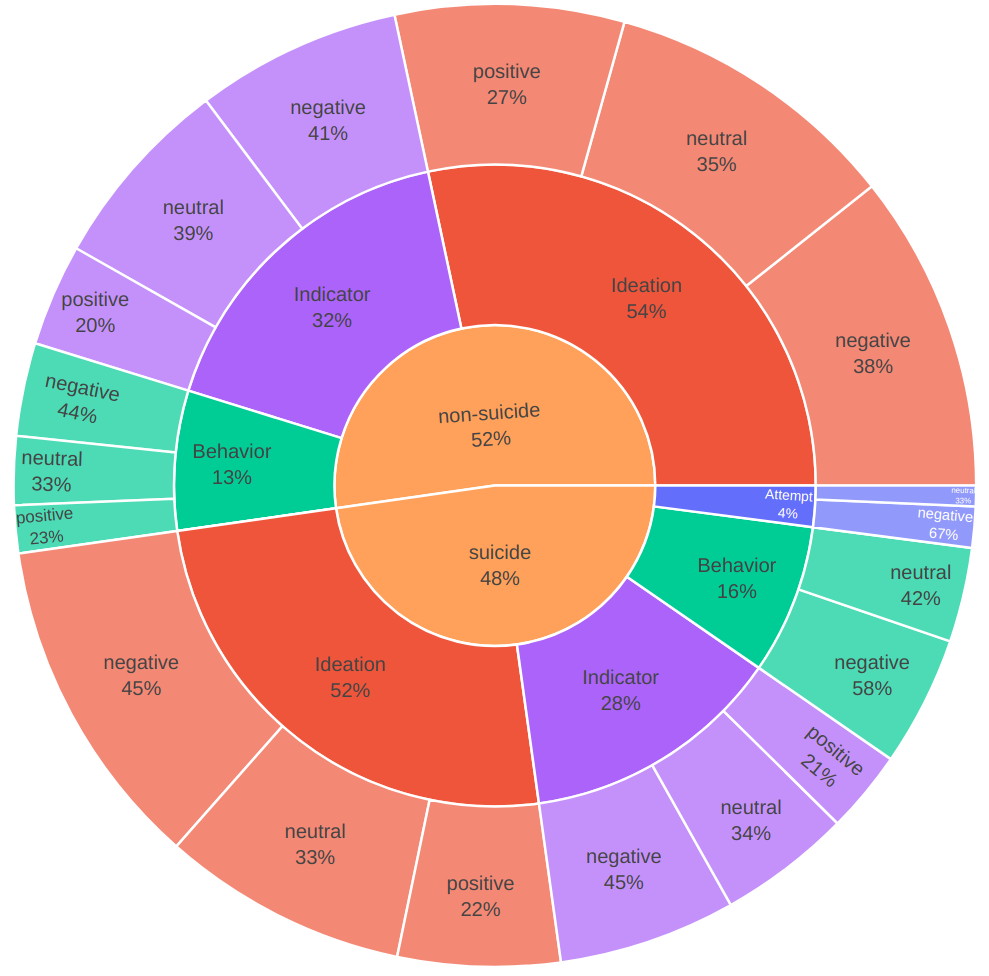
\includegraphics[width=\textwidth]{sentiment_sunburst.png}
    \caption{First subfigure.}
    \label{fig:first}
\end{subfigure}
\hfill
\begin{subfigure}{0.45\textwidth}
    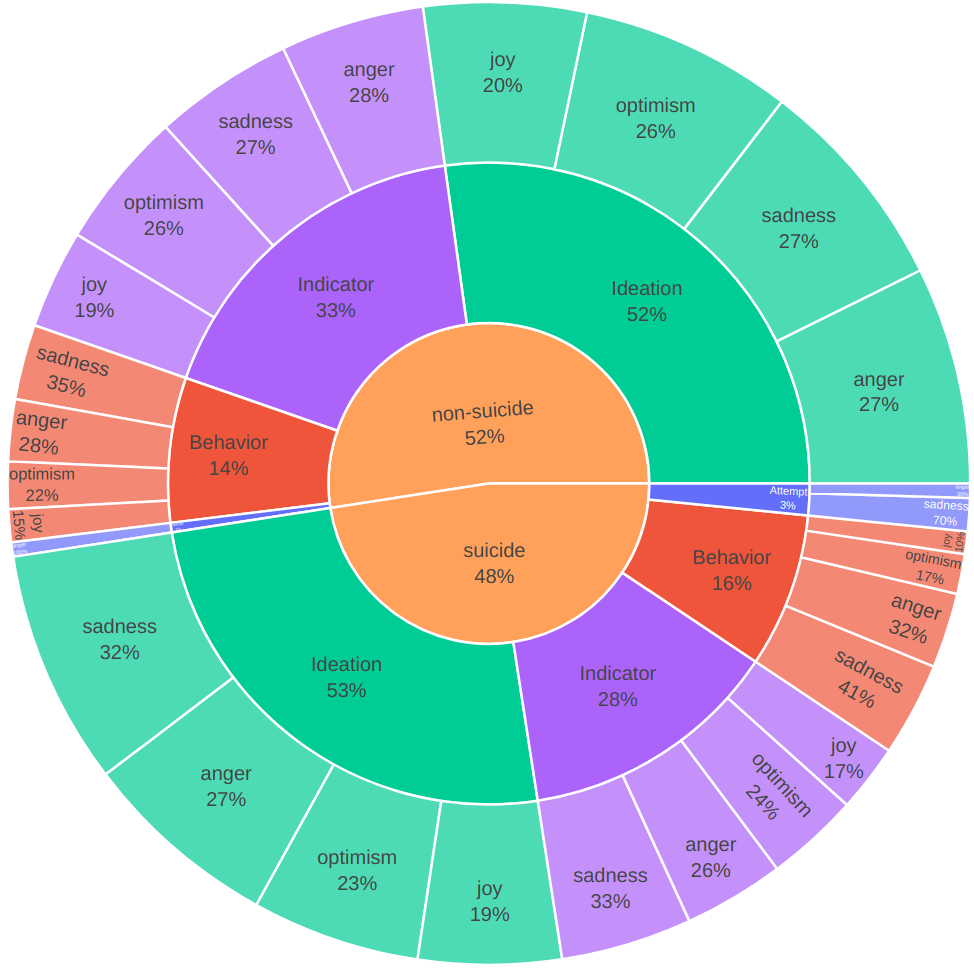
\includegraphics[width=\textwidth]{emotion_sunburst.png}
    \caption{Second subfigure.}
    \label{fig:second}
\end{subfigure}
        
\caption{Subreferences in \LaTeX.}
\label{fig:figures}
\end{figure}

\bibliographystyle{plain} % We choose the "plain" reference style
\bibliography{sn-bibliography} % Entries are in the refs.bib file
\end{document}
